% Author: Izaak Neutelings (September 2020)
% Inspiration: https://tex.stackexchange.com/questions/25531/adding-underbrace-in-tikz
\documentclass[border=3pt,tikz]{standalone}
\usepackage{physics}
\usepackage{tikz}
\usetikzlibrary{calc} % for pic
\usetikzlibrary{arrows.meta}
\usetikzlibrary{patterns}
\usetikzlibrary{angles,quotes} % for pic
\tikzset{>=latex} % for LaTeX arrow head

\colorlet{myred}{red!65!black}
%\colorlet{mylightblue}{blue!20}
\colorlet{mydarkblue}{blue!30!black}
\colorlet{xcol}{blue!70!black}
\colorlet{vcol}{green!70!black}
\colorlet{acol}{red!50!blue!80!black!80}
\tikzstyle{ground}=[preaction={fill,top color=black!10,bottom color=black!5,shading angle=20},
                    fill,pattern=north east lines,draw=none,minimum width=0.3,minimum height=0.6]
\tikzstyle{mass}=[line width=0.6,red!30!black,fill=red!40!black!10,rounded corners=1,
                  top color=red!40!black!20,bottom color=red!40!black!10,shading angle=20]
\tikzstyle{vector}=[->,very thick,xcol,line cap=round]
\tikzstyle{force}=[->,myred,thick,line cap=round]
\tikzstyle{Fproj}=[force,myred!40]
\tikzstyle{mydashed}=[dash pattern=on 2pt off 2pt]
\tikzstyle{smallarrow}=[{Latex[length=2,width=2]}-{Latex[length=2,width=2]}]
\newcommand{\vbF}{\vb{F}}
\def\tick#1#2{\draw[thick] (#1) ++ (#2:0.1) --++ (#2-180:0.2)} %0.03*\xmax



\begin{document}

% WORK DIAGONAL
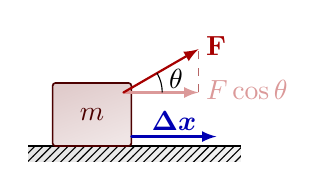
\begin{tikzpicture}
    \def\W{2.7}  % ground width
    \def\D{0.2}  % ground depth
    \def\h{0.8}  % mass height
    \def\w{1.0}  % mass width
    \def\F{1.1}  % force magnitude
    \def\ang{30} % angle force
    \coordinate (F0) at (0.4*\w,0.85*\h);
    \coordinate (Fx) at ($(F0)+({\F*cos(\ang)},0)$);
    \coordinate (F)  at ($(F0)+(\ang:\F)$);
    \draw[ground] (-0.3*\W,0) rectangle++ (\W,-\D);
    \draw (-0.3*\W,0) --++ (\W,0);
    \draw[mass] (-\w/2,0) rectangle++ (\w,\h) node[midway] {$m$};
    \draw[force,xcol] (\w/2,0.15*\h) --++ (0.4*\W,0) node[midway,above=-1.5] {$\vb*{\Delta x}$};
    \draw[dashed,myred!80!black!60] (Fx) -- (F);
    \draw[Fproj] (F0) -- (Fx) node[above=1,right=-1] {$F\cos\theta$}; %\vu{x}
    \draw[force] (F0) -- (F)  node[above=1,right=-1] {$\vbF$};
    \draw pic["$\theta$",draw=black,angle radius=14,angle eccentricity=1.4] {angle=Fx--F0--F};
\end{tikzpicture}

\end{document}